
\section{Cascaded PID Control Loop}

The algorithm utilizes cascade Proportional–Integral–Derivative (PID) control loop to maintain balance and control the robot's movement in real time. The balancing is achieved by continuously monitoring and adjusting its state using sensor feedback. The key sensor inputs include the robot's pitch angle, gyro data and motor's encoder values, which provide information on the robot's orientation, angular velocities and position.The algorithm utilizes cascade PID control loops to maintain balance and control the robot's movement in real time. The approach includes computing control outputs for pitch, yaw, and position periodically, which are then used to adjust the motor speeds by sending corresponding pulse-width-modulation (PWM) signals to the motor driver (see Fig. \ref{fig:control-loop}).

\begin{figure}[h]
	\centering
	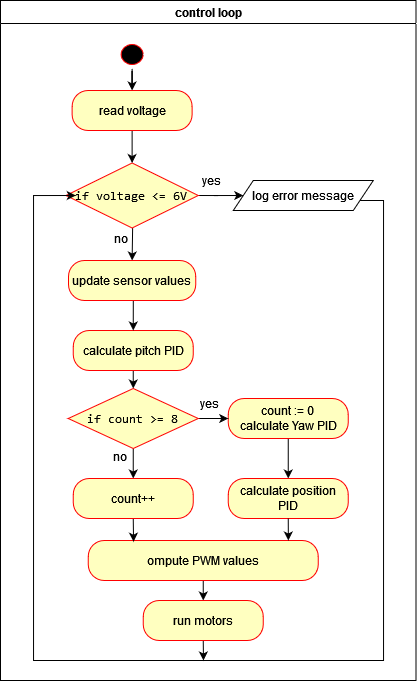
\includegraphics[width=0.5\linewidth]{assets/Control_Loop.png}
	\caption{A simplified block diagram of the control loop. }
	\label{fig:control-loop}
\end{figure}

As the pitch angle is more important for system stability, therefore it is updated more frequently (e.g. updated every cycle), while the PID output values for the yaw angle and position control are updated longer duration of time (e.g. after every 8th cycle).

\subsection{Basic PID Structure}
The PID controller output can be expressed mathematically as:

\begin{equation}
	u(t) = K_p e(t) + K_i \int_0^t e(\tau)d\tau + K_d \frac{d}{dt}e(t)
\end{equation}

Where:
\begin{itemize}
	\item $u(t)$ is the control signal
	\item $e(t)$ is the error signal
	\item $K_p$ is the proportional gain
	\item $K_i$ is the integral gain
	\item $K_d$ is the derivative gain
\end{itemize}



\subsection{Position Control Loop}
The outer loop manages the robot's position:

\begin{equation}
	\theta_{desired} = K_{px}(x_{desired} - x_{measured}) + K_{dx}\frac{d}{dt}(x_{desired} - x_{measured})
\end{equation}


\section{Implementation Considerations}
\subsection{Discrete Time Implementation}
For digital implementation, the PID controller is discretized:

\begin{equation}
	u[n] = K_p e[n] + K_i T_s \sum_{k=0}^n e[k] + K_d \frac{e[n] - e[n-1]}{T_s}
\end{equation}

Where $T_s$ is the sampling period.


\section{Tuning Methodology}
For tuning a general combination of Ziegler-Nichols method and practical tuning guidelines were used.
\subsection{Ziegler-Nichols Method}
The Ziegler-Nichols tuning method follows these steps:
\begin{enumerate}
	\item Set $K_i$ and $K_d$ to zero
	\item Increase $K_p$ until system oscillates with period $T_u$
	\item Record the ultimate gain $K_u$
	\item Calculate parameters:
	\begin{align*}
		K_p &= 0.6K_u \\
		T_i &= 0.5T_u \\
		T_d &= 0.125T_u
	\end{align*}
\end{enumerate}

\subsection{Practical Tuning Guidelines}
The general tuning guidelines are as follows:

\begin{itemize}
	\item Begin with small $K_p$ (= 10)
	\item Add derivative term ($K_d = 0.1K_p$)
	\item Fine-tune until stable
\end{itemize}


\subsection{Pitch PID Control:}
The pitch control loop ensures the robot maintains its upright position. The primary objective of the pitch controller is to minimize the deviation of the robot's pitch angle from a set-point, which is ideally zero degrees (i.e., upright). The pitch control output is calculated using the PD algorithm, where the error is the difference between the current pitch angle and the desired pitch angle. 
\begin{equation}
	\tau_{\theta,pid} = K_{p\theta}({\theta_{desired} - \theta_{measured}}) + K_{d\theta}\frac{d}{dt}(\theta_{desired} - \theta_{measured})
\end{equation}

Below is its code implementation:
\begin{lstlisting}[style=cppstyle]
inline void runPitchControl() {
	// Compute balance control output
	pitch_pid_output = kp_balance * (kalman.angle - 0) 
	+ kd_balance * (gyro_x  - 0);
}
\end{lstlisting}

\begin{itemize}
	\item \textbf{Proportional (P):} The proportional term is based on the current error (the pitch angle deviation from the desired value). A higher proportional gain causes the robot to respond more aggressively to larger deviations.
	\item \textbf{Derivative (D):} The derivative term anticipates future errors by considering the rate of change of the error (pitch angular velocity deviation from desired value). It provides a damping effect, which helps to reduce overshooting and oscillations.
	\item \textbf{Integral (I):} Because the system is inherently unstable when at desired upright position (steady state error can never be zero) thus adding the integral term is unnecessary. 
	
\end{itemize}

The output of the pitch PD controller ($\text{pitch\_pid\_output}$) is then used to adjust the robot's motor speeds to counteract any tilting or imbalance.

\subsection{Yaw Control:}
Yaw control is responsible for controlling the robot's rotational movement around its vertical axis. The yaw PID controller computes the control output based on the robot's angular velocity, which is measured by the gyroscope along the z-axis. The yaw control adjusts the motor speeds to achieve the desired rotational velocity, ensuring the robot maintains a stable heading.
\begin{equation}
	\tau_{\phi,pid} = K_{d\phi}\frac{d}{dt}(\phi_{desired} - \phi_{measured})
\end{equation}


Below is its code implementation:
\begin{lstlisting}[style=cppstyle]
inline void runYawControl(){
	yaw_pid_output = kd_turn * gyro_z;
}
\end{lstlisting}

Similar to pitch control, the yaw controller follows the PID principles:
\begin{itemize}
	\item \textbf{Proportional (P):} In order to calculate yaw angle, a high computational overhead is required, while yaw angle is not critical for balancing thus the proportional term is ignored.
	\item \textbf{Integral (I):} As the yaw angle is not calculated, therefore the integral term cannot be calculated as well.
	\item \textbf{Derivative (D):} The derivative term mitigates any excessive rate of change in yaw, preventing oscillations in the robot's rotation.
\end{itemize}

The yaw PID output ($\text{yaw\_pid\_output}$) is then combined with the pitch and position control outputs to compute the final motor PWM values.

\subsection{Position Control:}
Position control is implemented to ensure the robot moves smoothly and accurately along a path or to a target location. The encoder feedback from the left and right wheels is used to calculate the robot's displacement and speed. The position PID controller adjusts the motor speeds to minimize the error in position and velocity.
\begin{equation}
	\tau_{x,pid} = K_{px}(x_{desired} - x_{measured}) + K_{dx}\frac{d}{dt}(x_{desired} - x_{measured})
\end{equation}

Below is its code implementation:
\begin{lstlisting}[style=cppstyle]
inline void runPositionControl(){
	double encoder_speed = (left_encoder_position + right_encoder_position) * 0.5
	robot_position += encoder_speed;
	robot_position = constrain(robot_position, -3000, 3000);
	position_pid_output = - ki_position * robot_position - kd_position * encoder_speed;
}
\end{lstlisting}

To prevent integral windup:
\begin{equation}
	u_{limited} = \begin{cases}
		3000 & \text{if } u > 3000 \\
		u & \text{if } -3000 \leq u \leq 3000 \\
		-3000 & \text{if } u < -3000
	\end{cases}
\end{equation}

\begin{itemize}
	\item \textbf{Proportional (P):} The proportional term helps correct any immediate error in position by adjusting the motor speeds in response to the current position error.
	\item \textbf{Integral (I):} The integral term addresses any accumulated error in position that may arise due to external factors like friction or uneven terrain.
	\item \textbf{Derivative (D):} Because the position control does not require fast settling time, thus derivative term can be ignored in favour of faster calculation time.
	
\end{itemize}

The position control output ($\text{position\_pid\_output}$) is also factored into the final PWM values for motor control.

\subsection{Combining Control Outputs}

The final motor control is achieved by combining the outputs from all three PID controllers. The outputs from the pitch, yaw, and position PID controllers are used to calculate the motor speeds, which determine the robot's motion. Specifically, the following equation is used to compute the PWM values for the left and right motors:

\begin{align}
	\tau_{left,motor} &= \tau_{\theta,pid} - \tau_{\phi,pid} - \tau_{x,pid} \\
	\tau_{right,motor} &= \tau_{\theta,pid} + \tau_{\phi,pid} - \tau_{x,pid}
\end{align}

Below is its code implementation:
\begin{lstlisting}[style=cppstyle]
pwm_left = pitch_pid_output - yaw_pid_output - position_pid_output;
pwm_right = pitch_pid_output + yaw_pid_output - position_pid_output;
\end{lstlisting}

These calculated PWM values are then sent to the motor drivers to adjust the robot's movement and balance.

\subsection{Conclusion}

The use of PID controllers for pitch, yaw, and position control enables the robot to maintain balance and navigate effectively. The proportional, integral, and derivative terms in each PID loop allow the system to respond to real-time errors, minimize steady-state deviations, and anticipate future errors, leading to smooth and precise control of the robot's motion. The integration of these PID controllers is fundamental to the robot's stability and performance.

